\chapter{任务二:发音与听觉感知}
\label{chap:task2}

\section{语音的谐波 harmonics}

\begin{figure}[!htp]
  \centering
  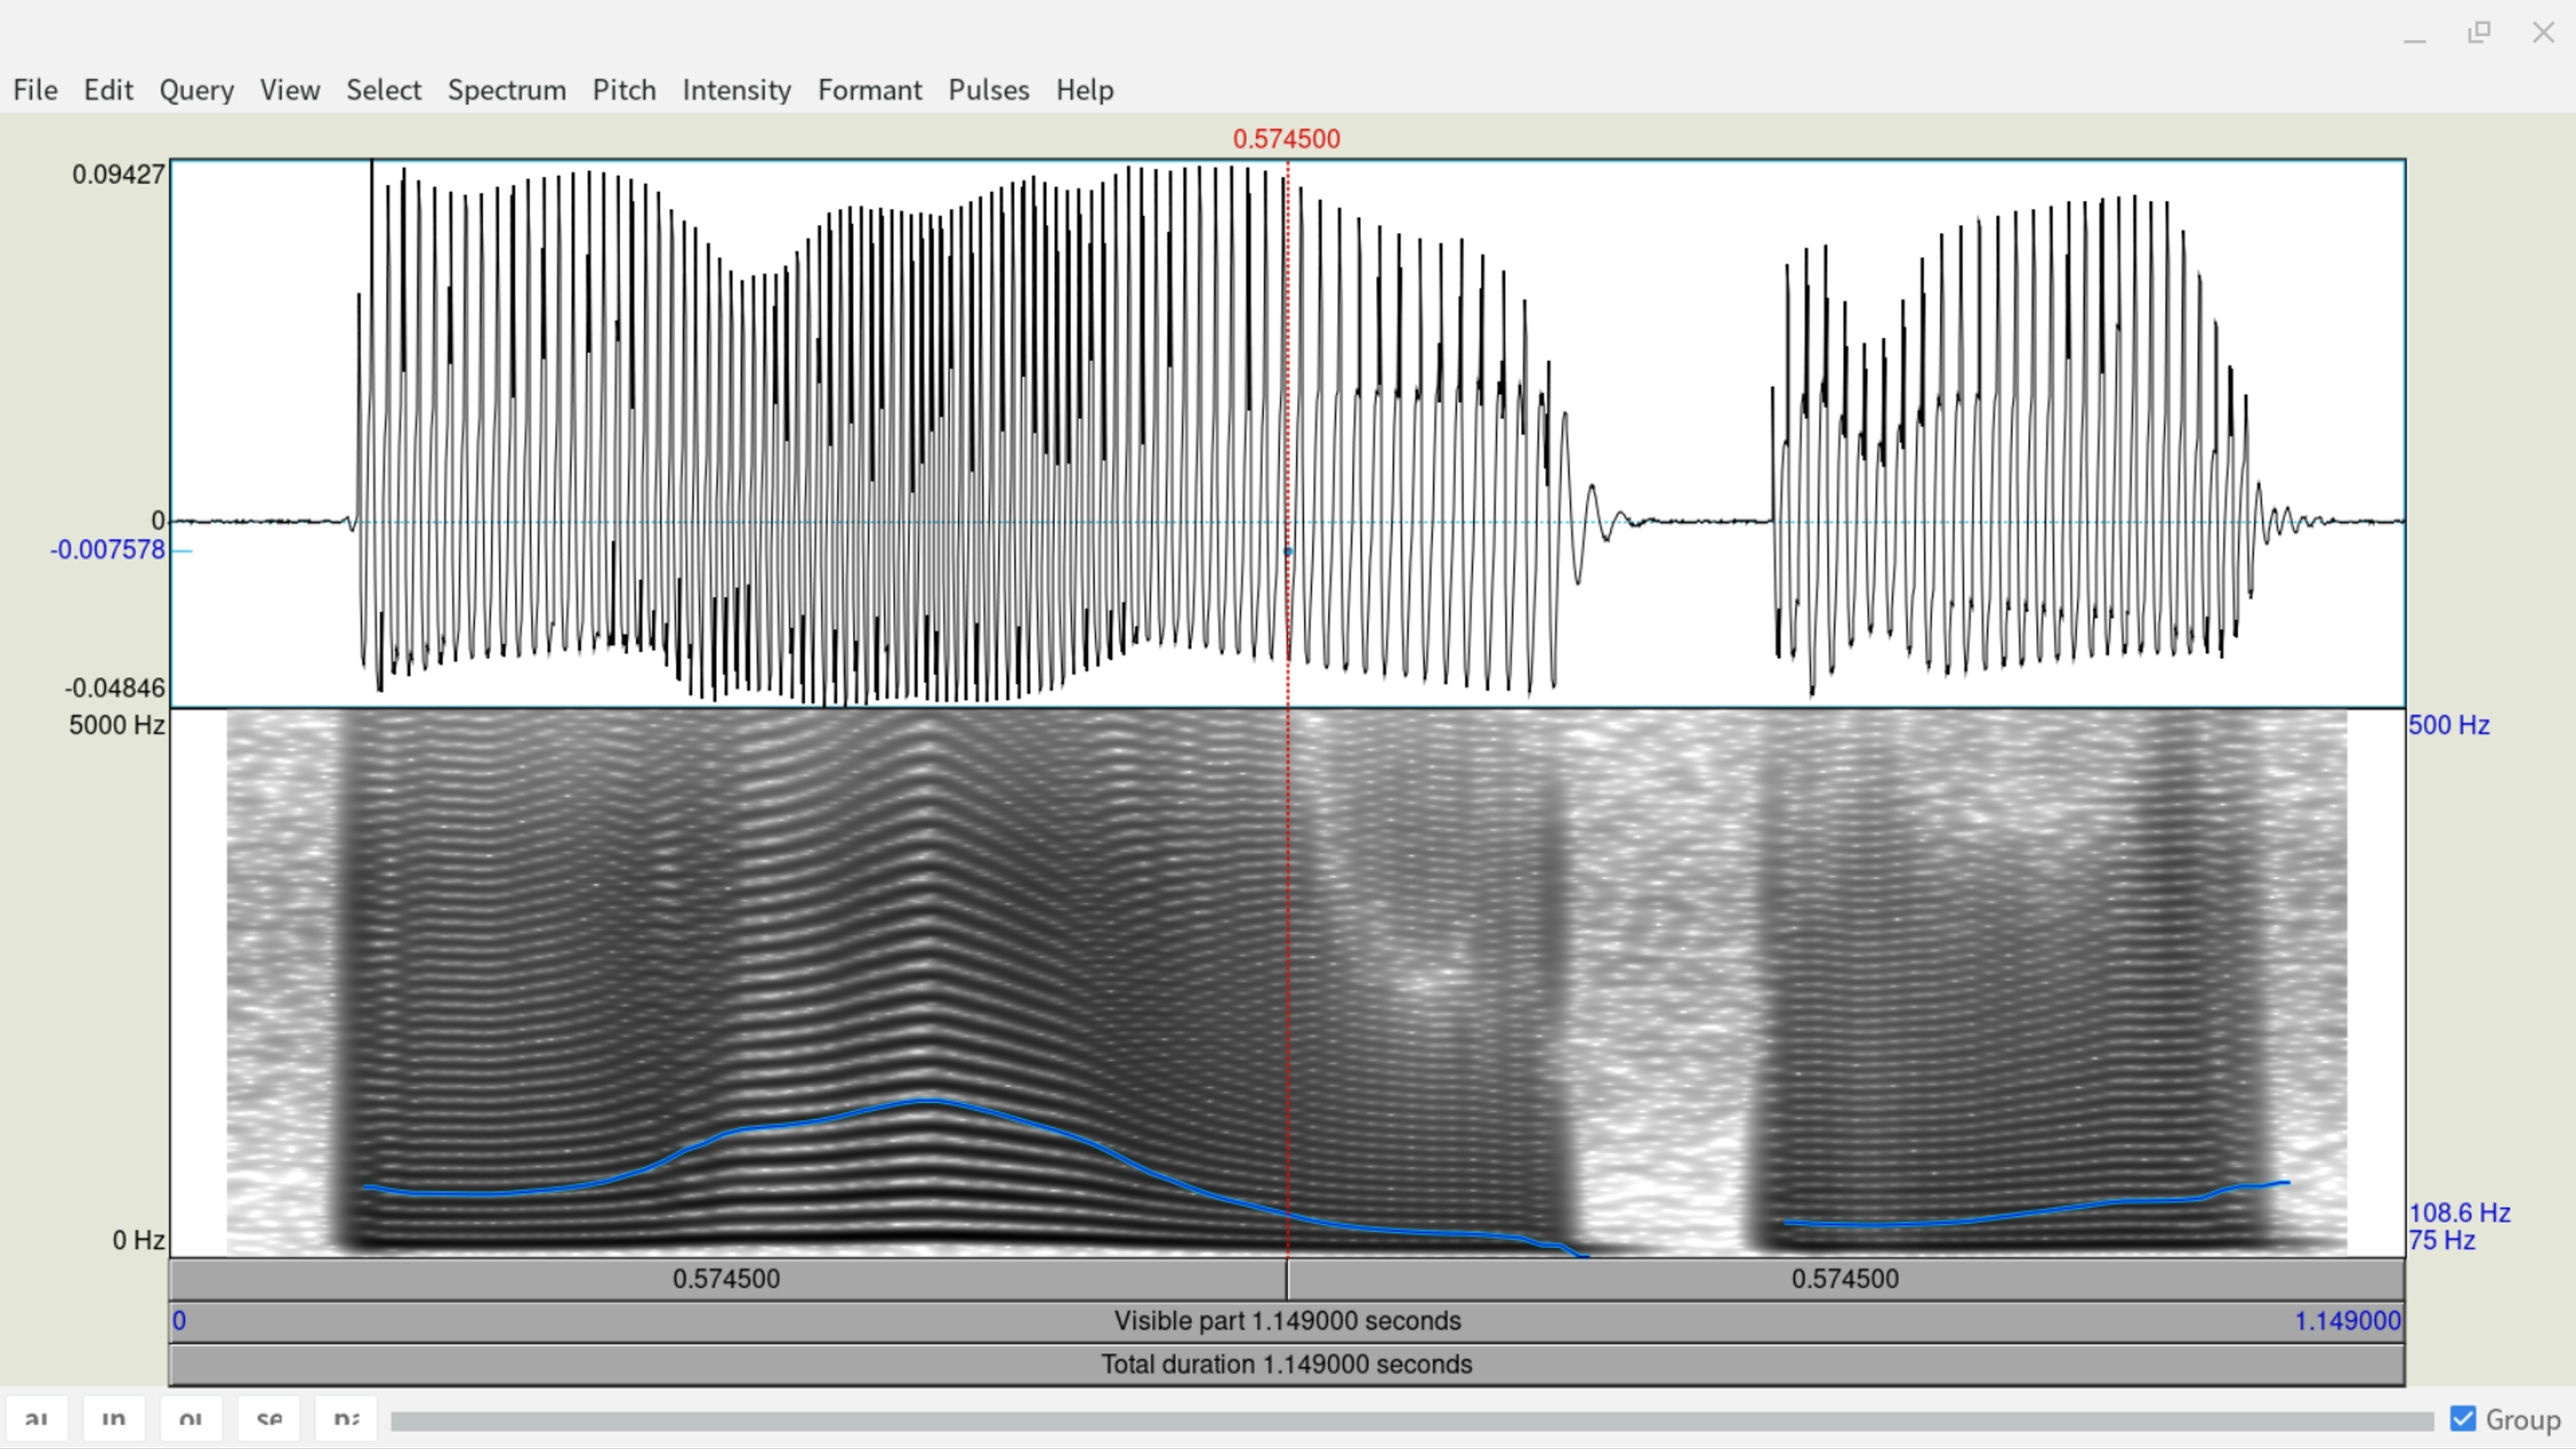
\includegraphics[width=.8\columnwidth]{harmonics.png}
  \caption{谐波}
  \label{fig:harmonics}
\end{figure}

从波形图中我们很难看出语音的谐波分量,不过我们可以通过语谱图轻松地看出语音的谐波及其能量。
不过 Praat 默认的参数设置($N = 5$ ms 的宽带语谱图)使得我们依然不能轻松地从语谱图中找出各个谐波分量。
我们只需要更改语谱图设置,把窗长调整到 $30$ ms,这时候,我们会发现语谱图中有非常多的细条纹。
当我们固定到某个时间刻度 $t$ 时,我们可以看出其频谱离散的,且是等距的,这就是谐波信号。
从频率最低的基频 $F_0$ 开始,所有谐波分量都是基频的整数倍。
并且谐波分量随着频率的增大,能量是逐渐减小的。

\begin{figure}[htp]
  \begin{center}
    \subfloat[语音信号波形]{%
        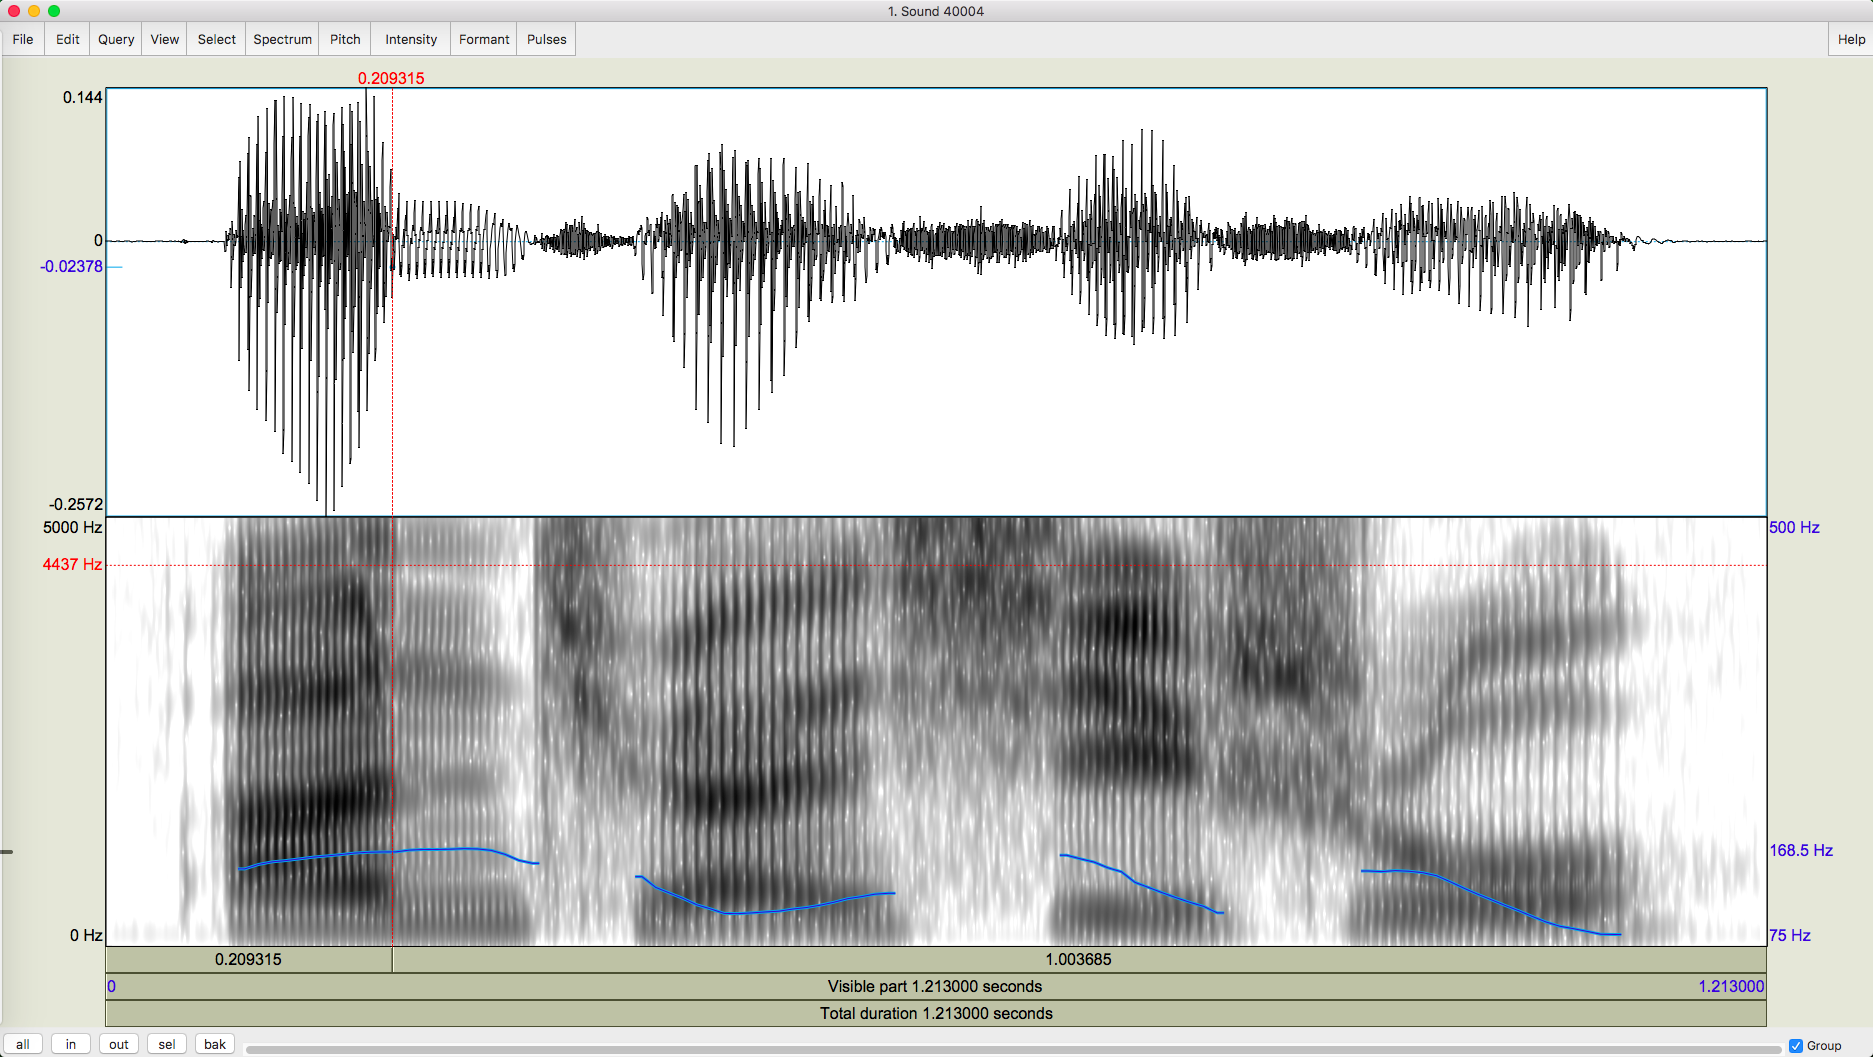
\includegraphics[clip,width=.8\columnwidth]{waveform_speech.png}%
    }

    \subfloat[EGG信号波形]{%
        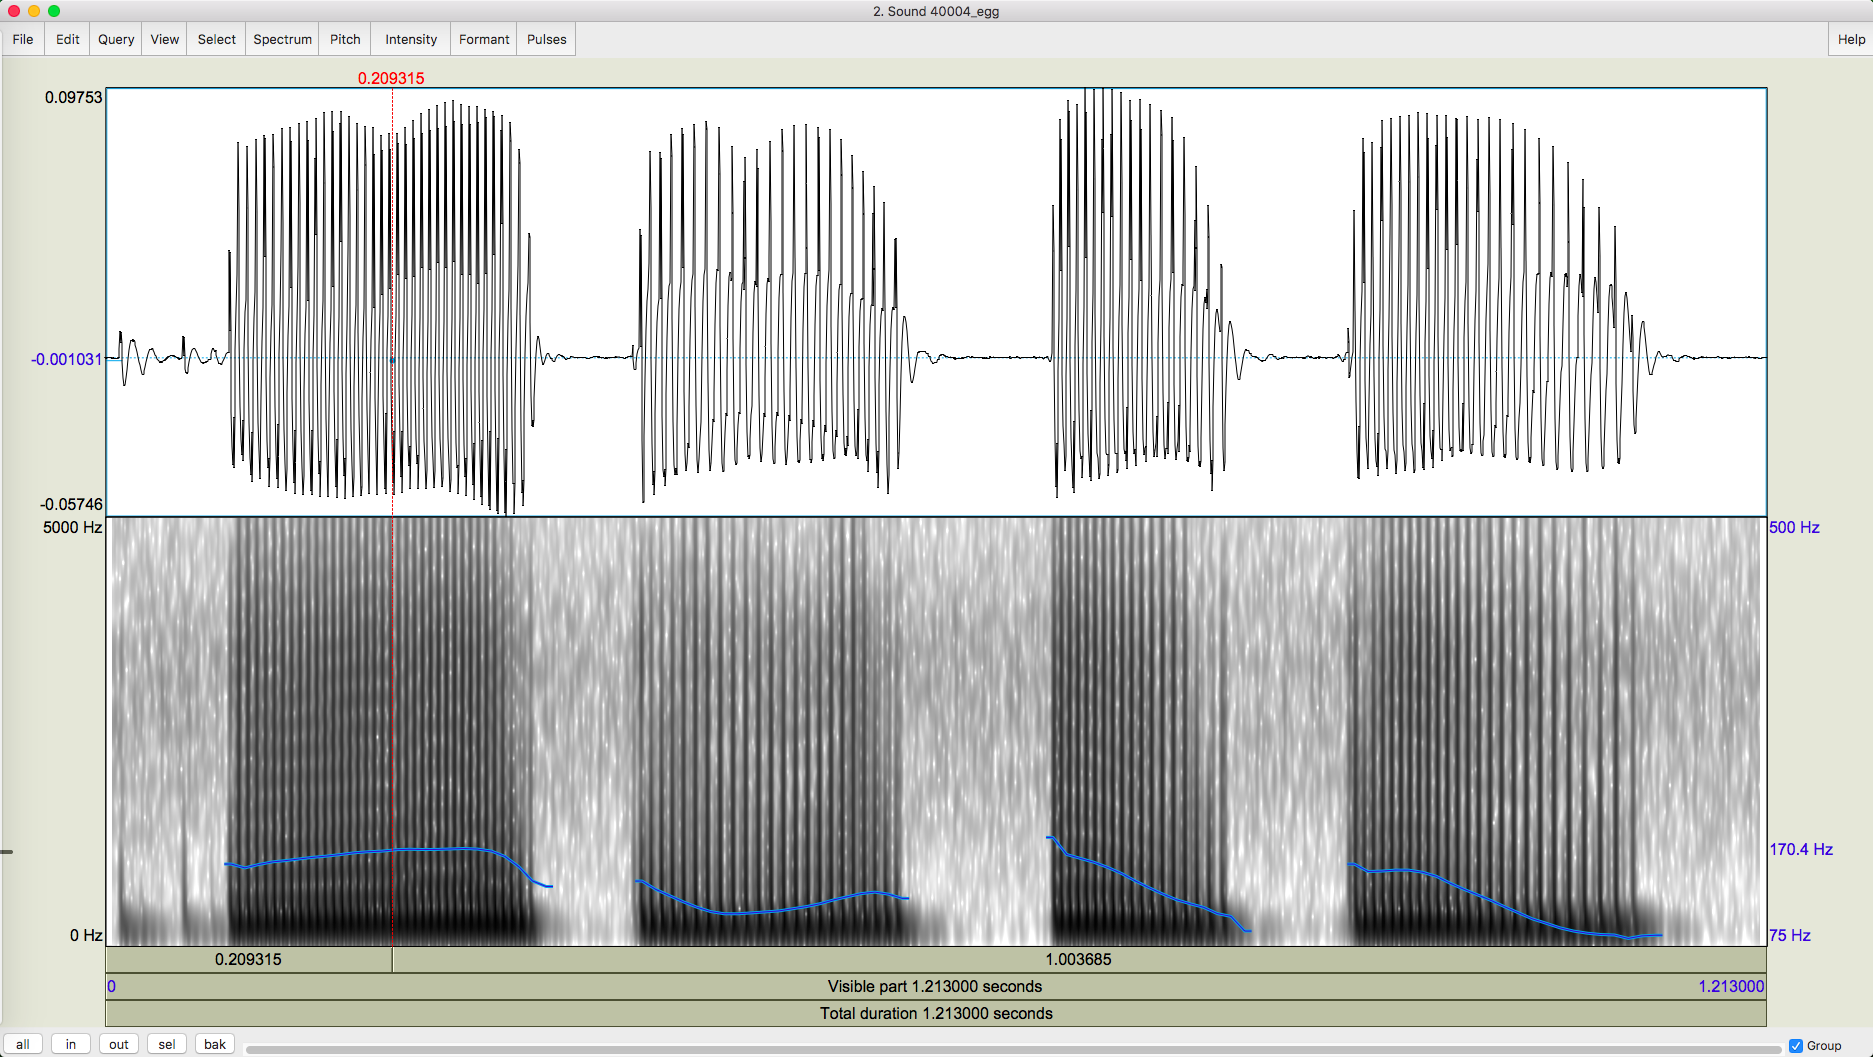
\includegraphics[clip,width=.8\columnwidth]{waveform_EGG.png}%
    }
  \end{center}
    \caption{比较 EGG 和语音信号波形}
    \label{fig:waveforms_speech_EGG}
\end{figure}

\section{比较 EGG 和语音信号波形}
在图~\ref{fig:waveforms_speech_EGG}中展示了语音信号波形和 EGG 信号波形的示例。
首先,EGG 和语音信号的时间长度是一样的,并且他们的清音和浊音的区域是一致的。
其次,音高(基频 $F_0$) 是一致的,虽然从波形图中无法直接看出来。

不同点在于,语音信号是 EGG 经过声道调制(Filter)后的输出。
EGG 信号在同一段浊音内表现出来的波形是比较规整的谐波信号。
具有较明显的周期性,也就是说其振幅的局部最大值的抖动较小。
并且对于清音部分,其能量很小,而且波动幅度也很小,说明噪声比较微弱。
其语谱图中的能量也是从基频到谐波分量,随着频率增加,能量逐渐下降。

\begin{figure}[htp]
  \begin{center}
  \subfloat[中性情绪]{%
    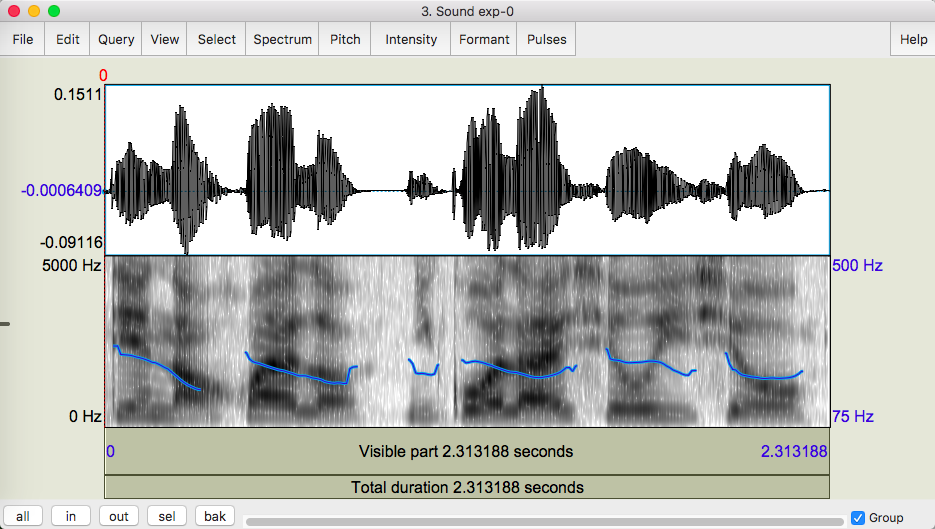
\includegraphics[clip,width=.6\columnwidth]{emotion_0.png}%
  }

  \subfloat[愤怒情绪]{%
    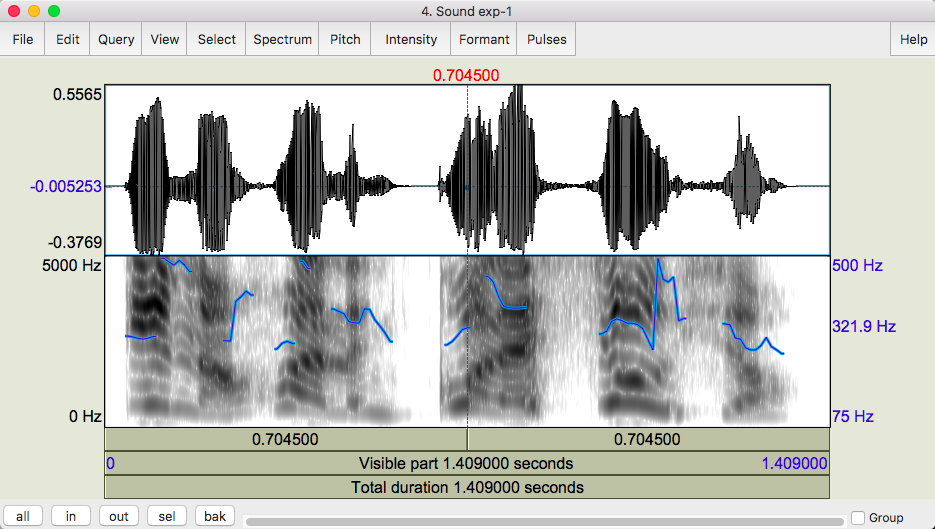
\includegraphics[clip,width=.6\columnwidth]{emotion_1.png}%
  }

  \subfloat[悲伤情绪]{%
    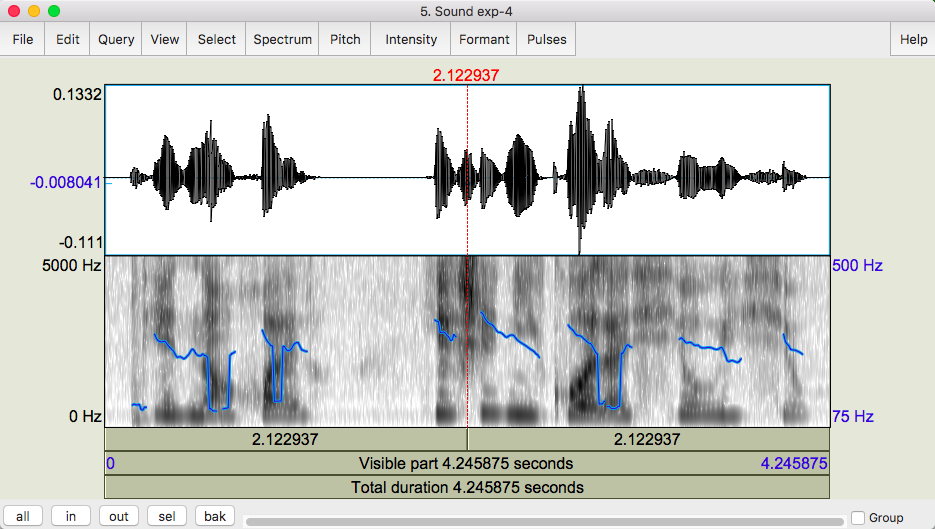
\includegraphics[clip,width=.6\columnwidth]{emotion_4.png}%
  }
  \end{center}
  \caption{不同情绪的基音轮廓}
  \label{fig:emotion}
\end{figure}

而语音信号表现为其抖动更加明显,并且在大时间尺度上没有明显的周期性,而在很小一段时间内其信号具有比较明显的周期性。
并且对于清音部分,可以明显看出其能量和波动都比 EGG 明显,说明噪声比较大。
从语谱图中我们可以看到,各个频率的能量分布与频率大小关系不大,不过具有比较明显的峰值特性,也就是说,语谱图中某一部分区域的能量比较大,而其他地方能量比较小,看起来有点像山峰山谷。

\section{不同情绪的基音轮廓}
可以从图~\ref{fig:emotion}中看出:

\begin{enumerate}
    \item 中性情绪的基音轮廓比较平滑,变化幅度不会很大。浊音和清音(没有基音轮廓的部分)的识别较好,间断点较少。
    \item 愤怒情绪的基音轮廓抖动比较大,有些部分浊音被错误识别为了清音,所以基音轮廓有更加多的间断点。同时,可以看出,其平均的基音频率都要高于中性情绪,基音轮廓中有许多上升的部分。听该段音频的时候明显感觉声音起伏落差明显,而且很急促。
    \item 悲伤情绪的基音轮廓抖动同样也比较大,也有一部分浊音被错误识别为清音的情况,不过间断点略少于愤怒情绪。同样的,其平均基音频率要低于中性情绪,其基音轮廓中有许多下降的部分。听的时候也明显感觉声音要低沉很多。
\end{enumerate}

从图中我们还可以看出,除了三种情绪的语音信号的基音轮廓不一样之外,他们的语谱图也有着明显的不一样。
也就是说这三种语音在发音的时候,他们不仅声门波不一样,他们的声道对语音信号的调制作用也是不一样的。
语谱图不一样同样也代表了共振峰是不一样的。
此外,因为基音轮廓不一样,所以脉冲是不一样的,并且由基频决定的谐波也是不一样的。
基本上,这三种语音信号,除了清音浊音的分布差不多(因为说的内容都是一样的几个字),其他许多声学特征都有明显差别,比如它们之间的振幅(能量)的差别很挺大的。
不过因为语速会有区别,所以它们的浊音持续时间也会有所区别。

\begin{figure}[htp]
  \begin{center}
  \subfloat[陈述语气]{%
    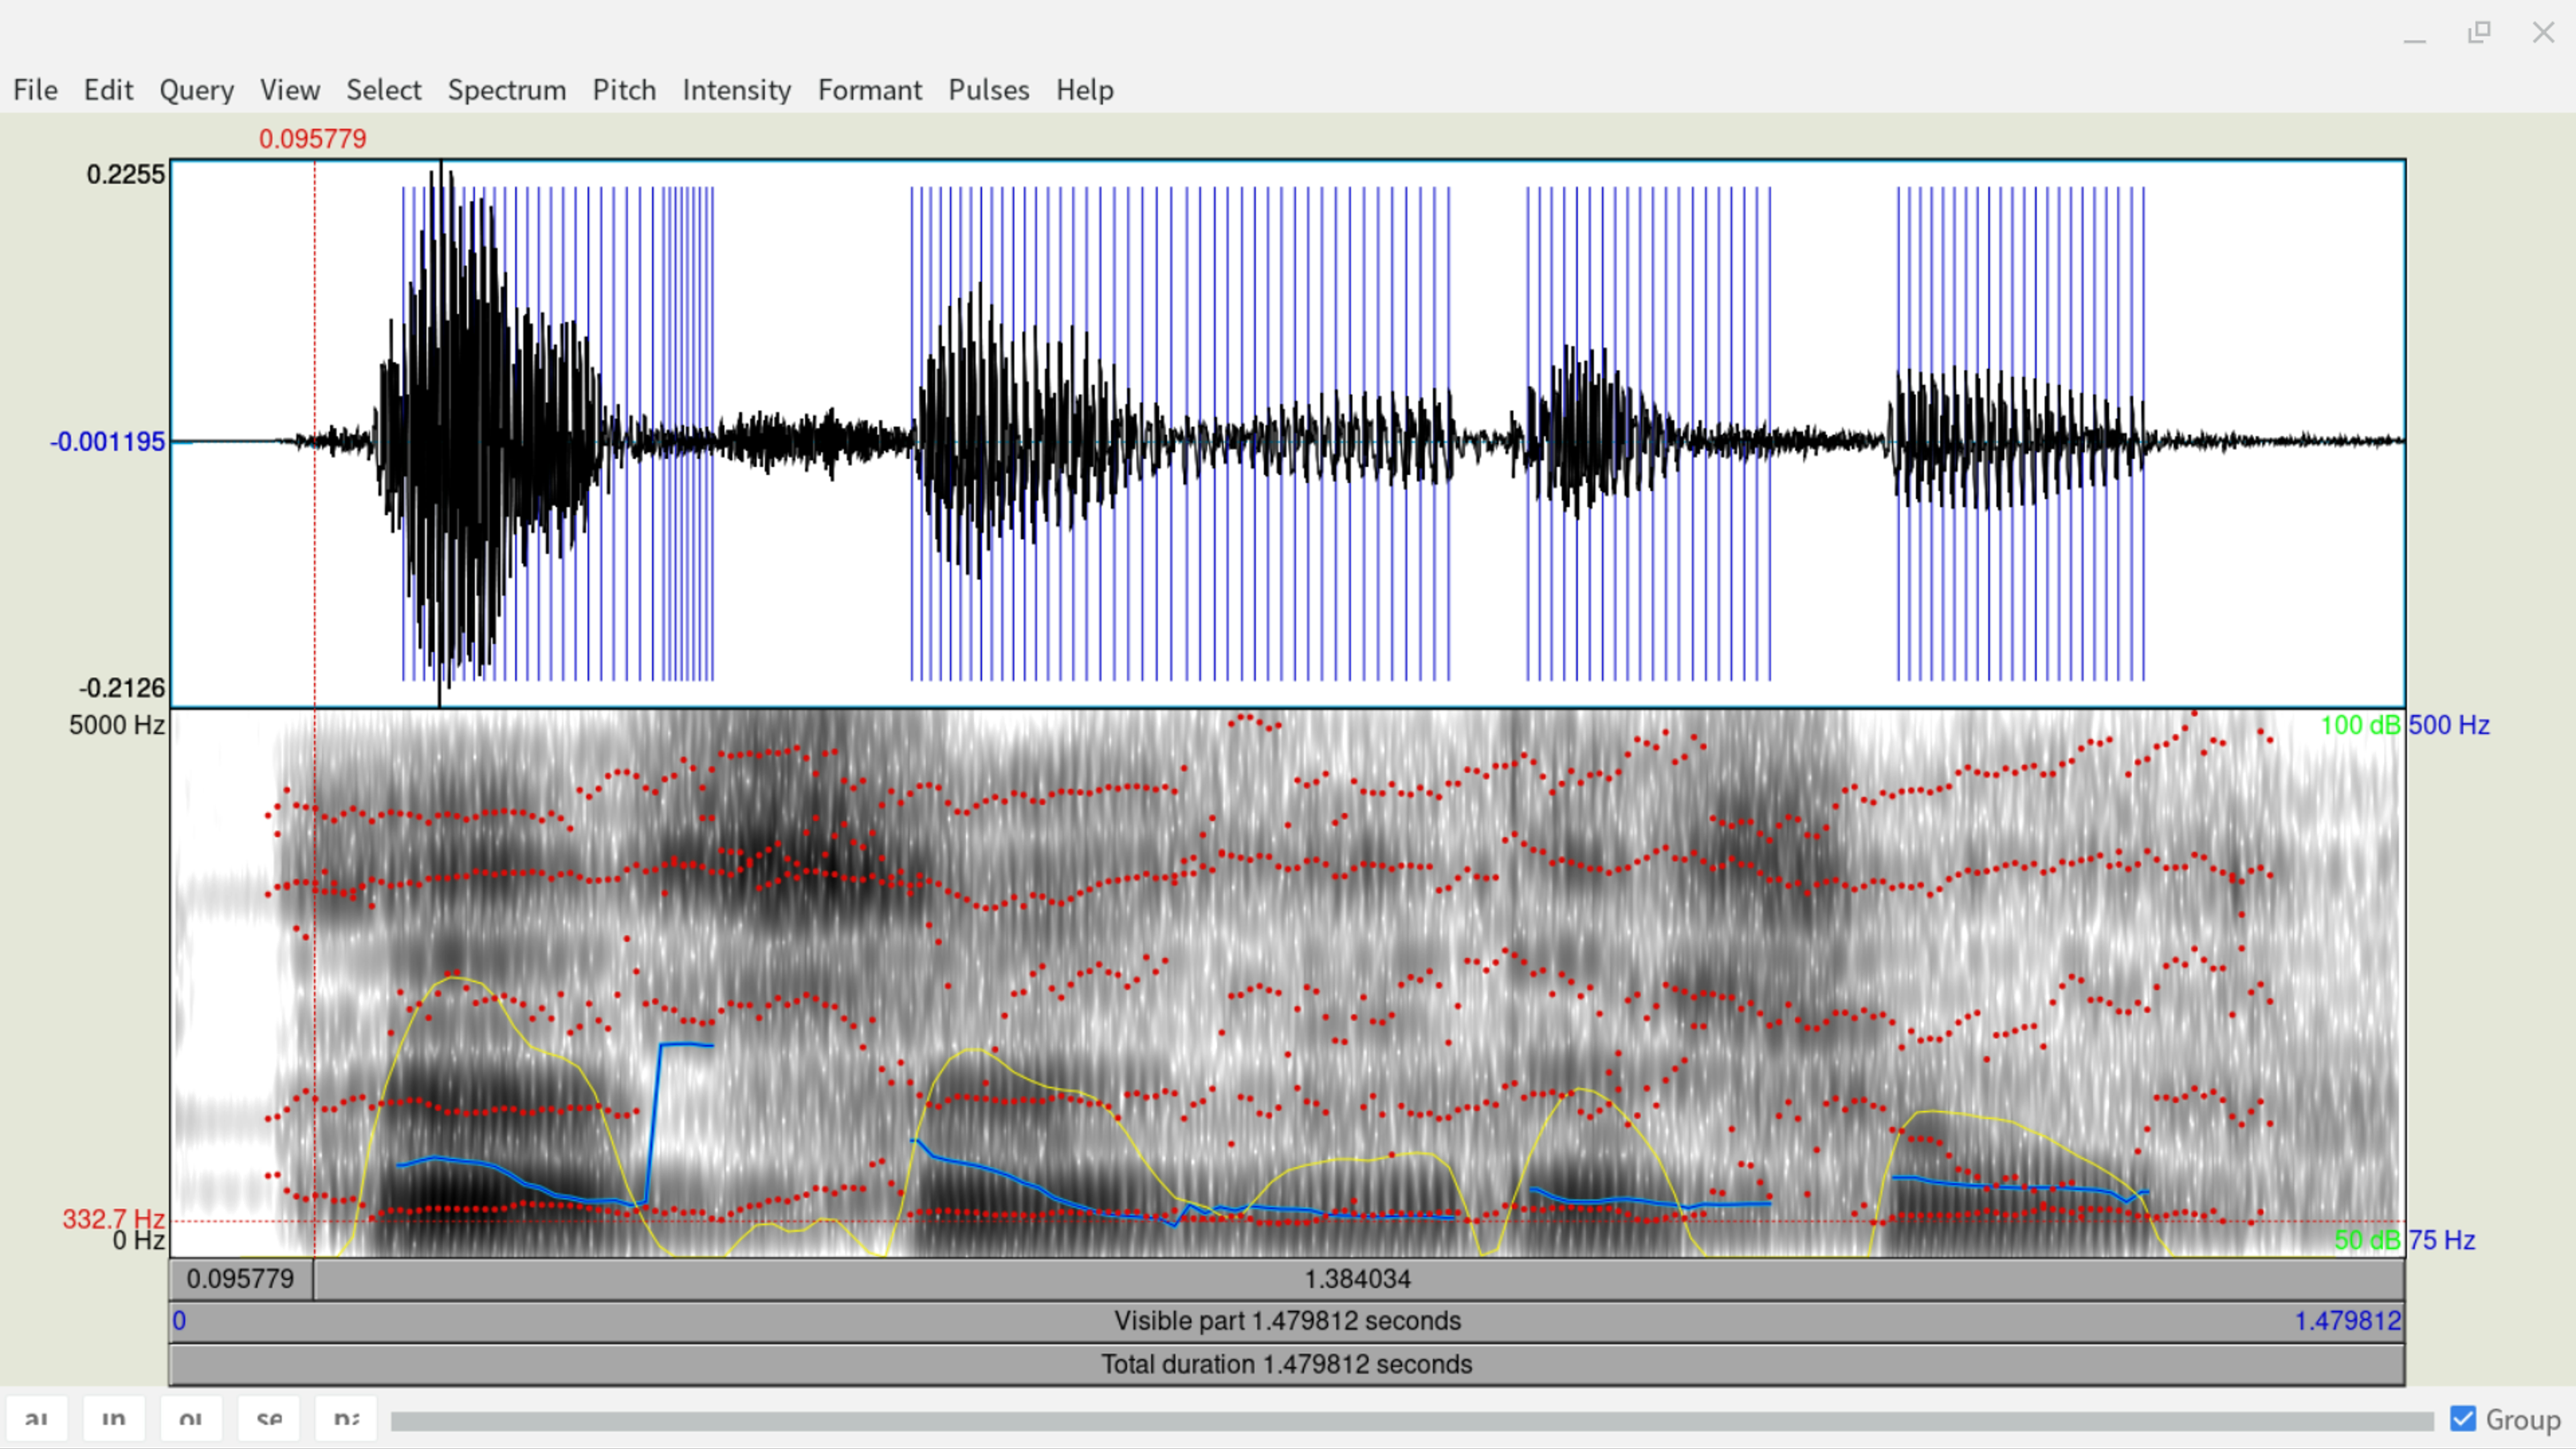
\includegraphics[clip,width=.6\columnwidth]{book_declaration.png}%
  }

  \subfloat[疑问语气]{%
    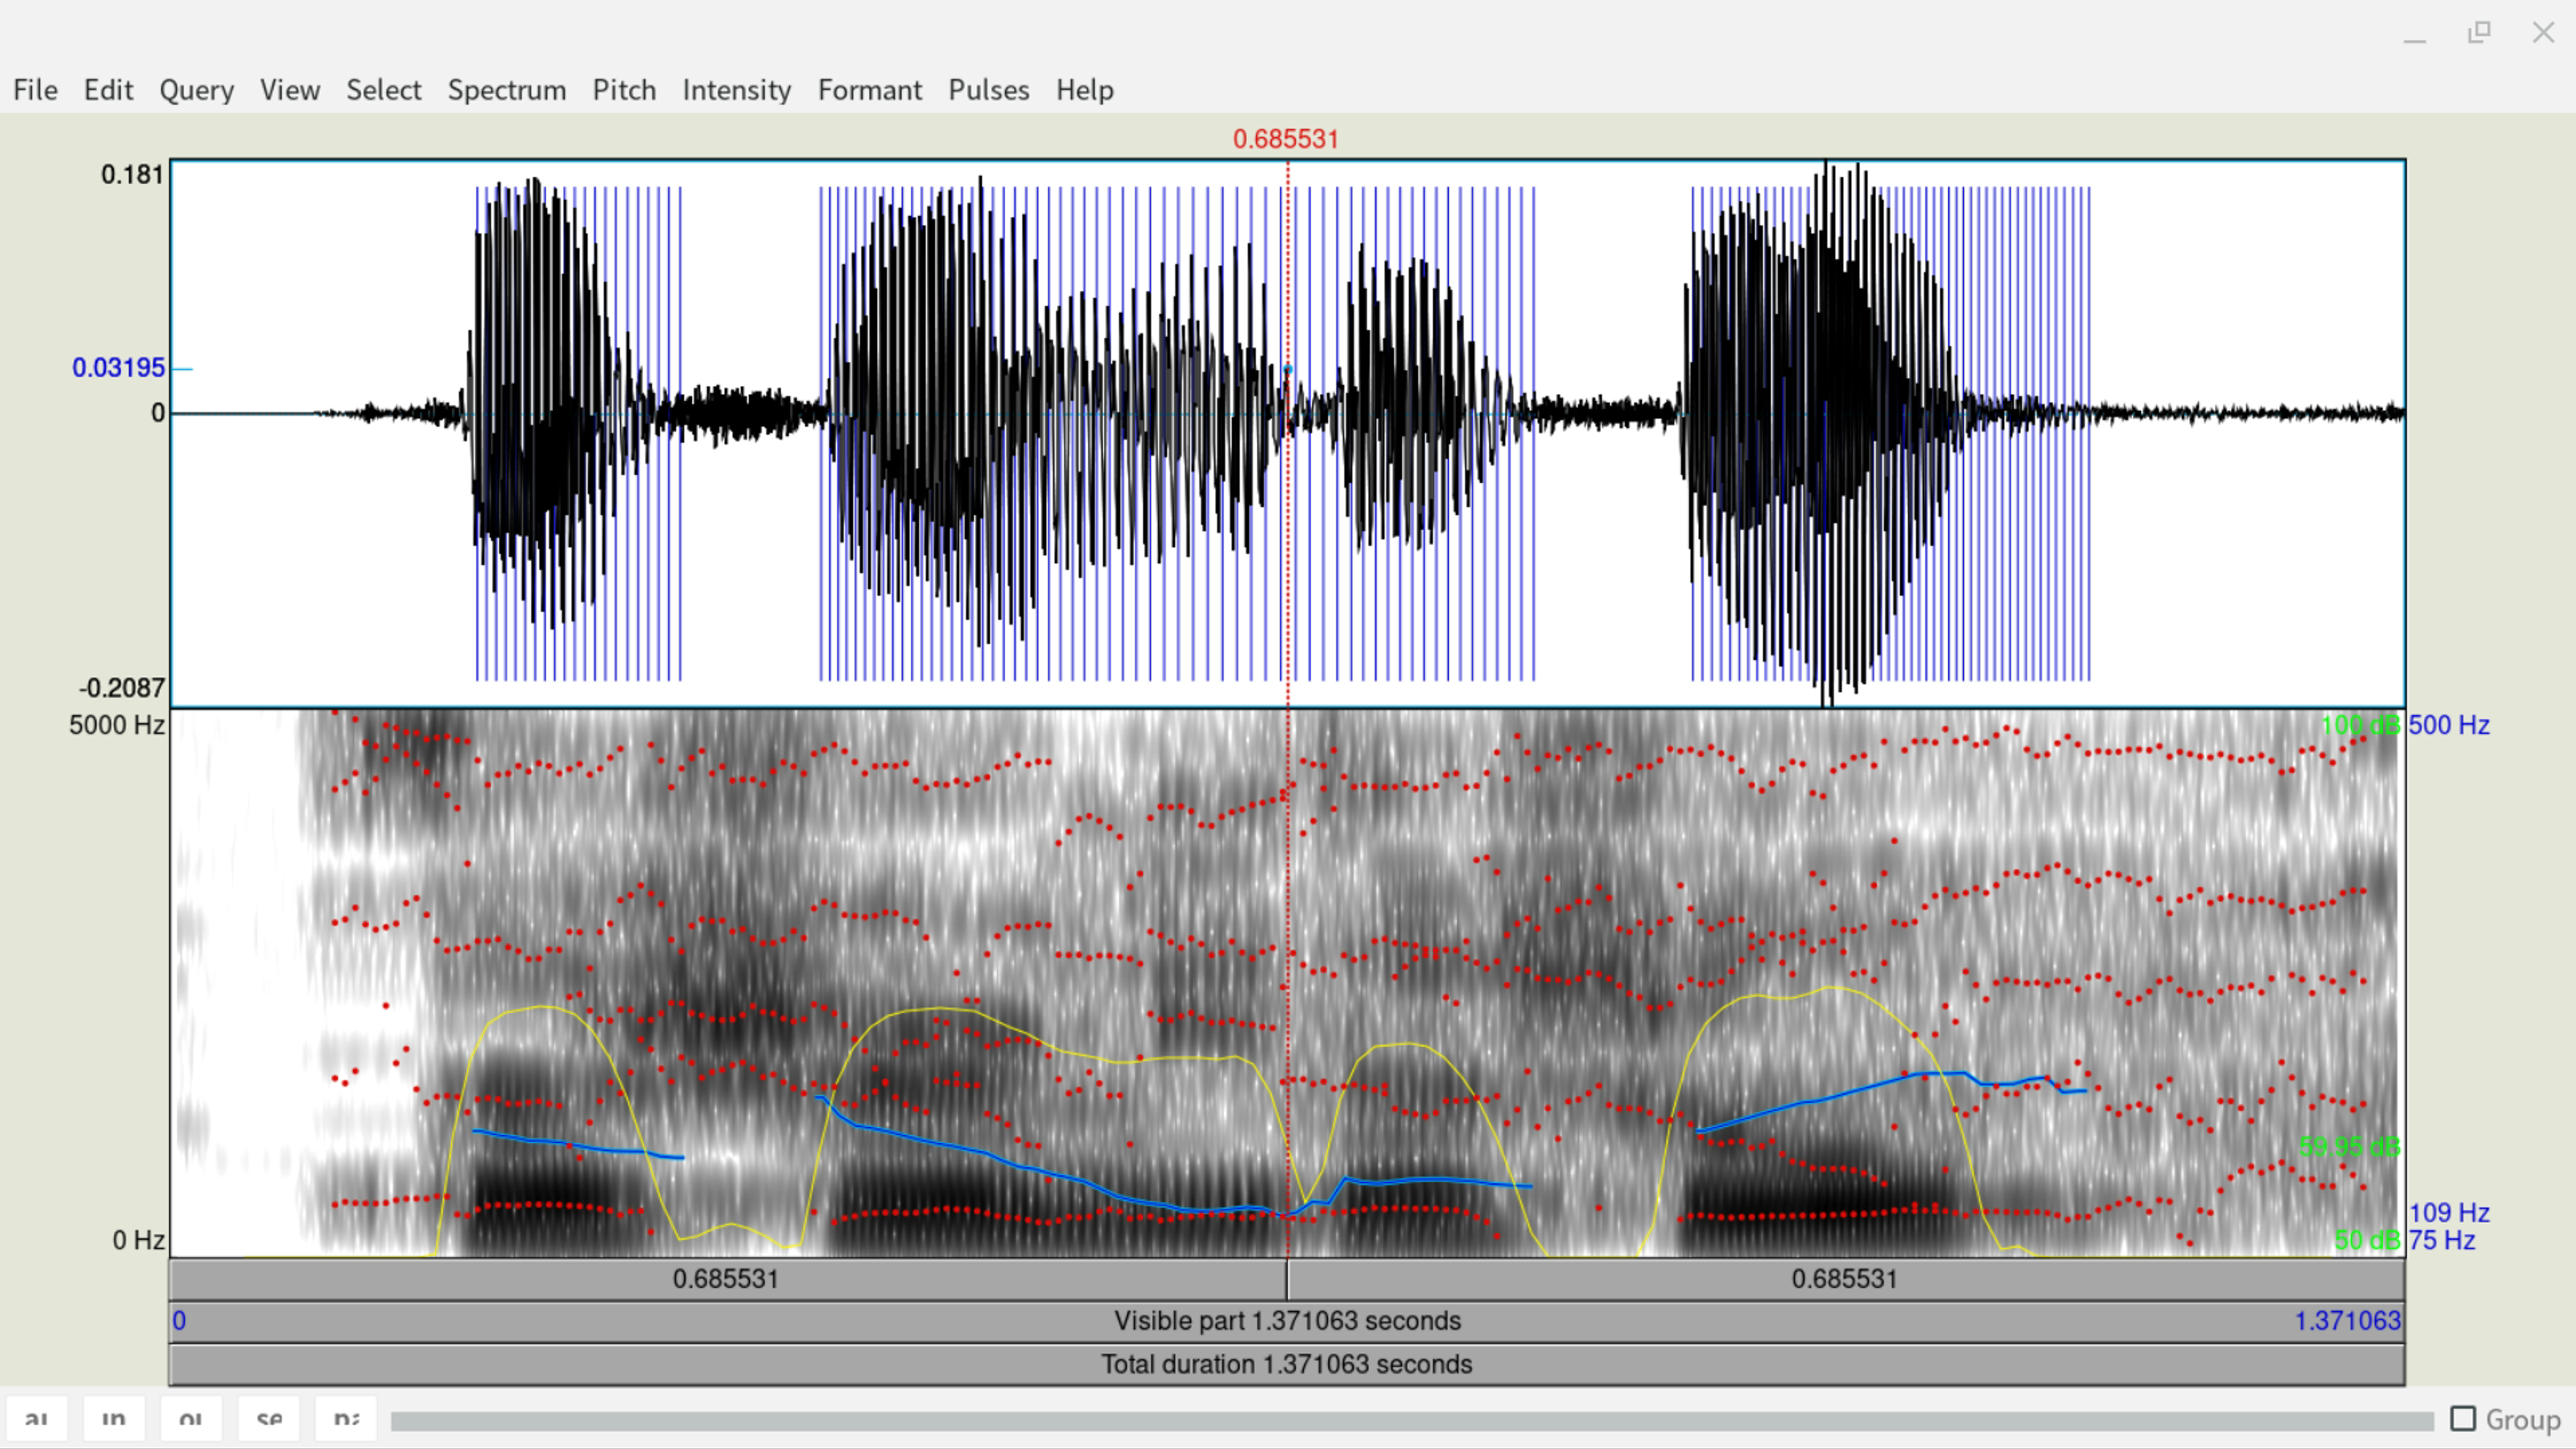
\includegraphics[clip,width=.6\columnwidth]{book_question.png}%
  }
  \end{center}
  \caption{不同语气的基音轮廓}
  \label{fig:book}
\end{figure}

\section{不同语气的基音轮廓}
因为不同情绪的声音同样语气也会有区别,所以不同语气的基音轮廓的区别也类似于不同情绪。参考图~\ref{fig:book},具体来说有以下一些差异:

\begin{enumerate}
\item \textbf{陈述语气}:对每一个浊音单元,我们可以看出基音轮廓都是下降的,属于降调语气(忽略第一个浊音单元后面突然上升的那一部分,那部分是识别错误)。
\item \textbf{疑问语气}:对前半部分的浊音单元,我们可以看出基音轮廓都是下降的,因为前面几个字基本上是陈述语气。而后半部分的浊音单元,尤其是最后一个字——\textbf{书}——的时候,它的基音轮廓是明显的升调的,因为此时是疑问语气。
\end{enumerate}

\begin{figure}[htp]
  \begin{center}
  \subfloat[宽带语谱图($N = 5$ ms)]{%
    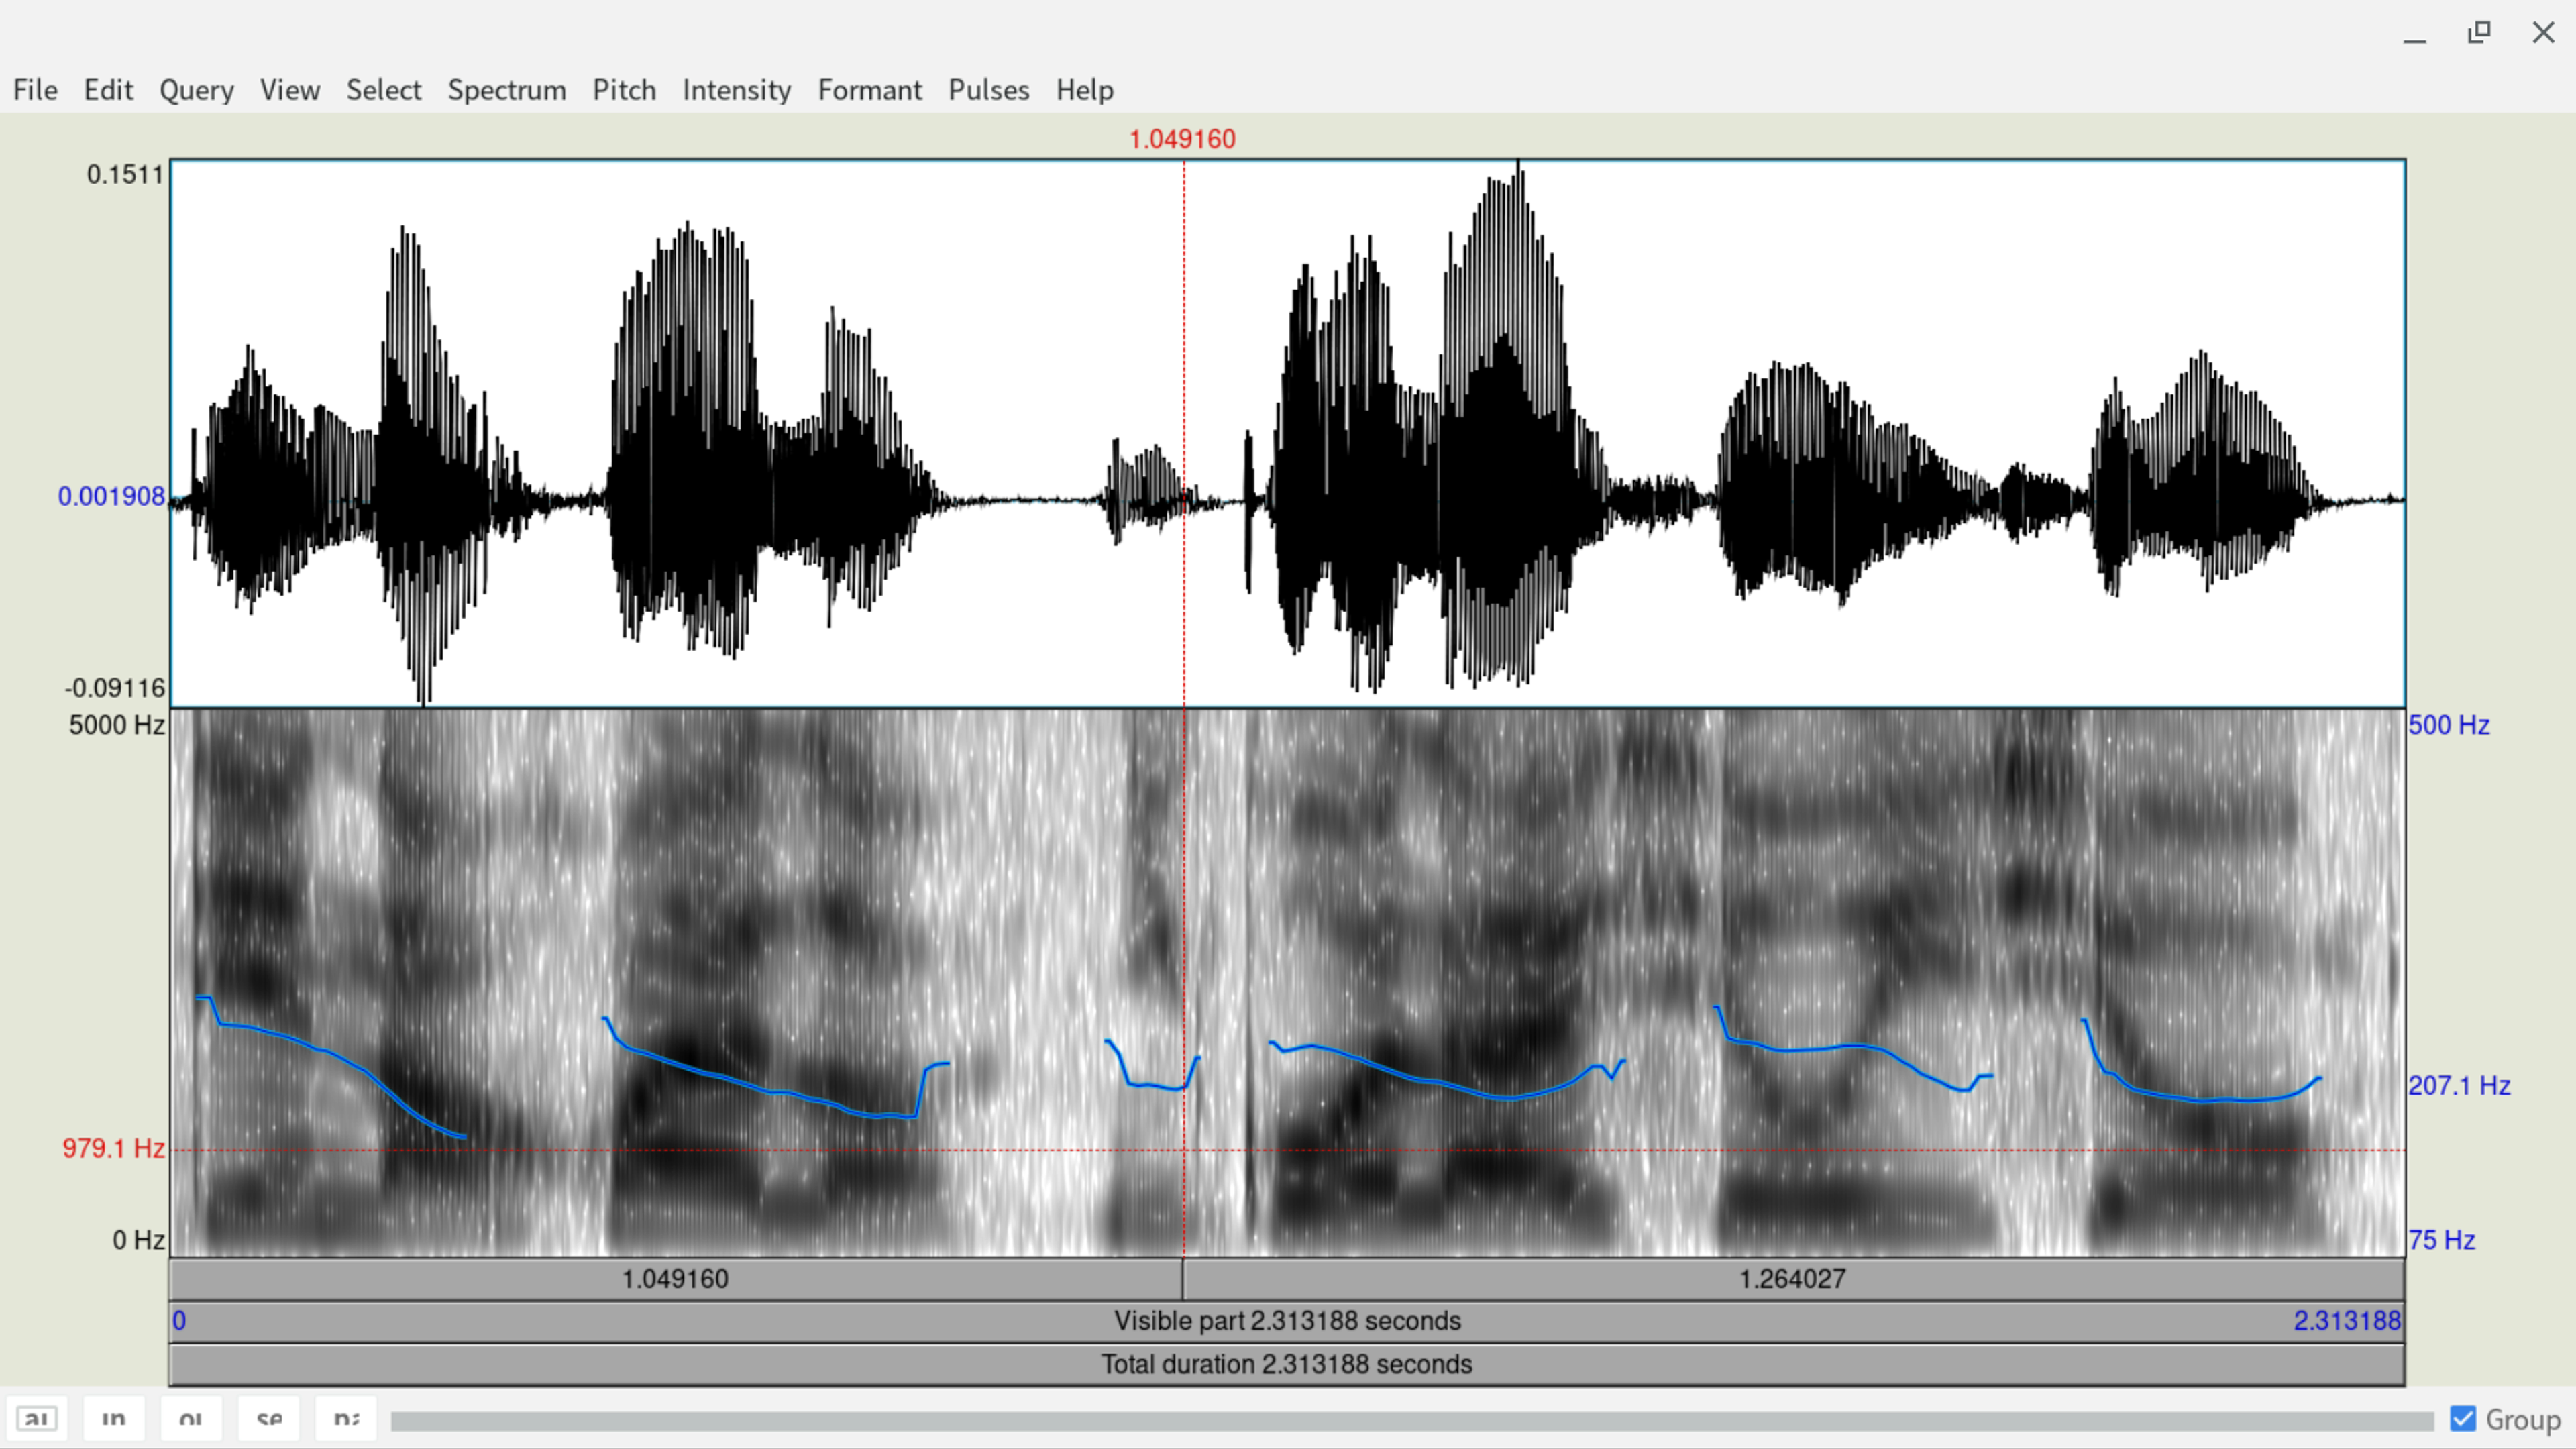
\includegraphics[clip,width=.6\columnwidth]{wideband.png}%
  }

  \subfloat[窄带语谱图($N = 30$ ms)]{%
    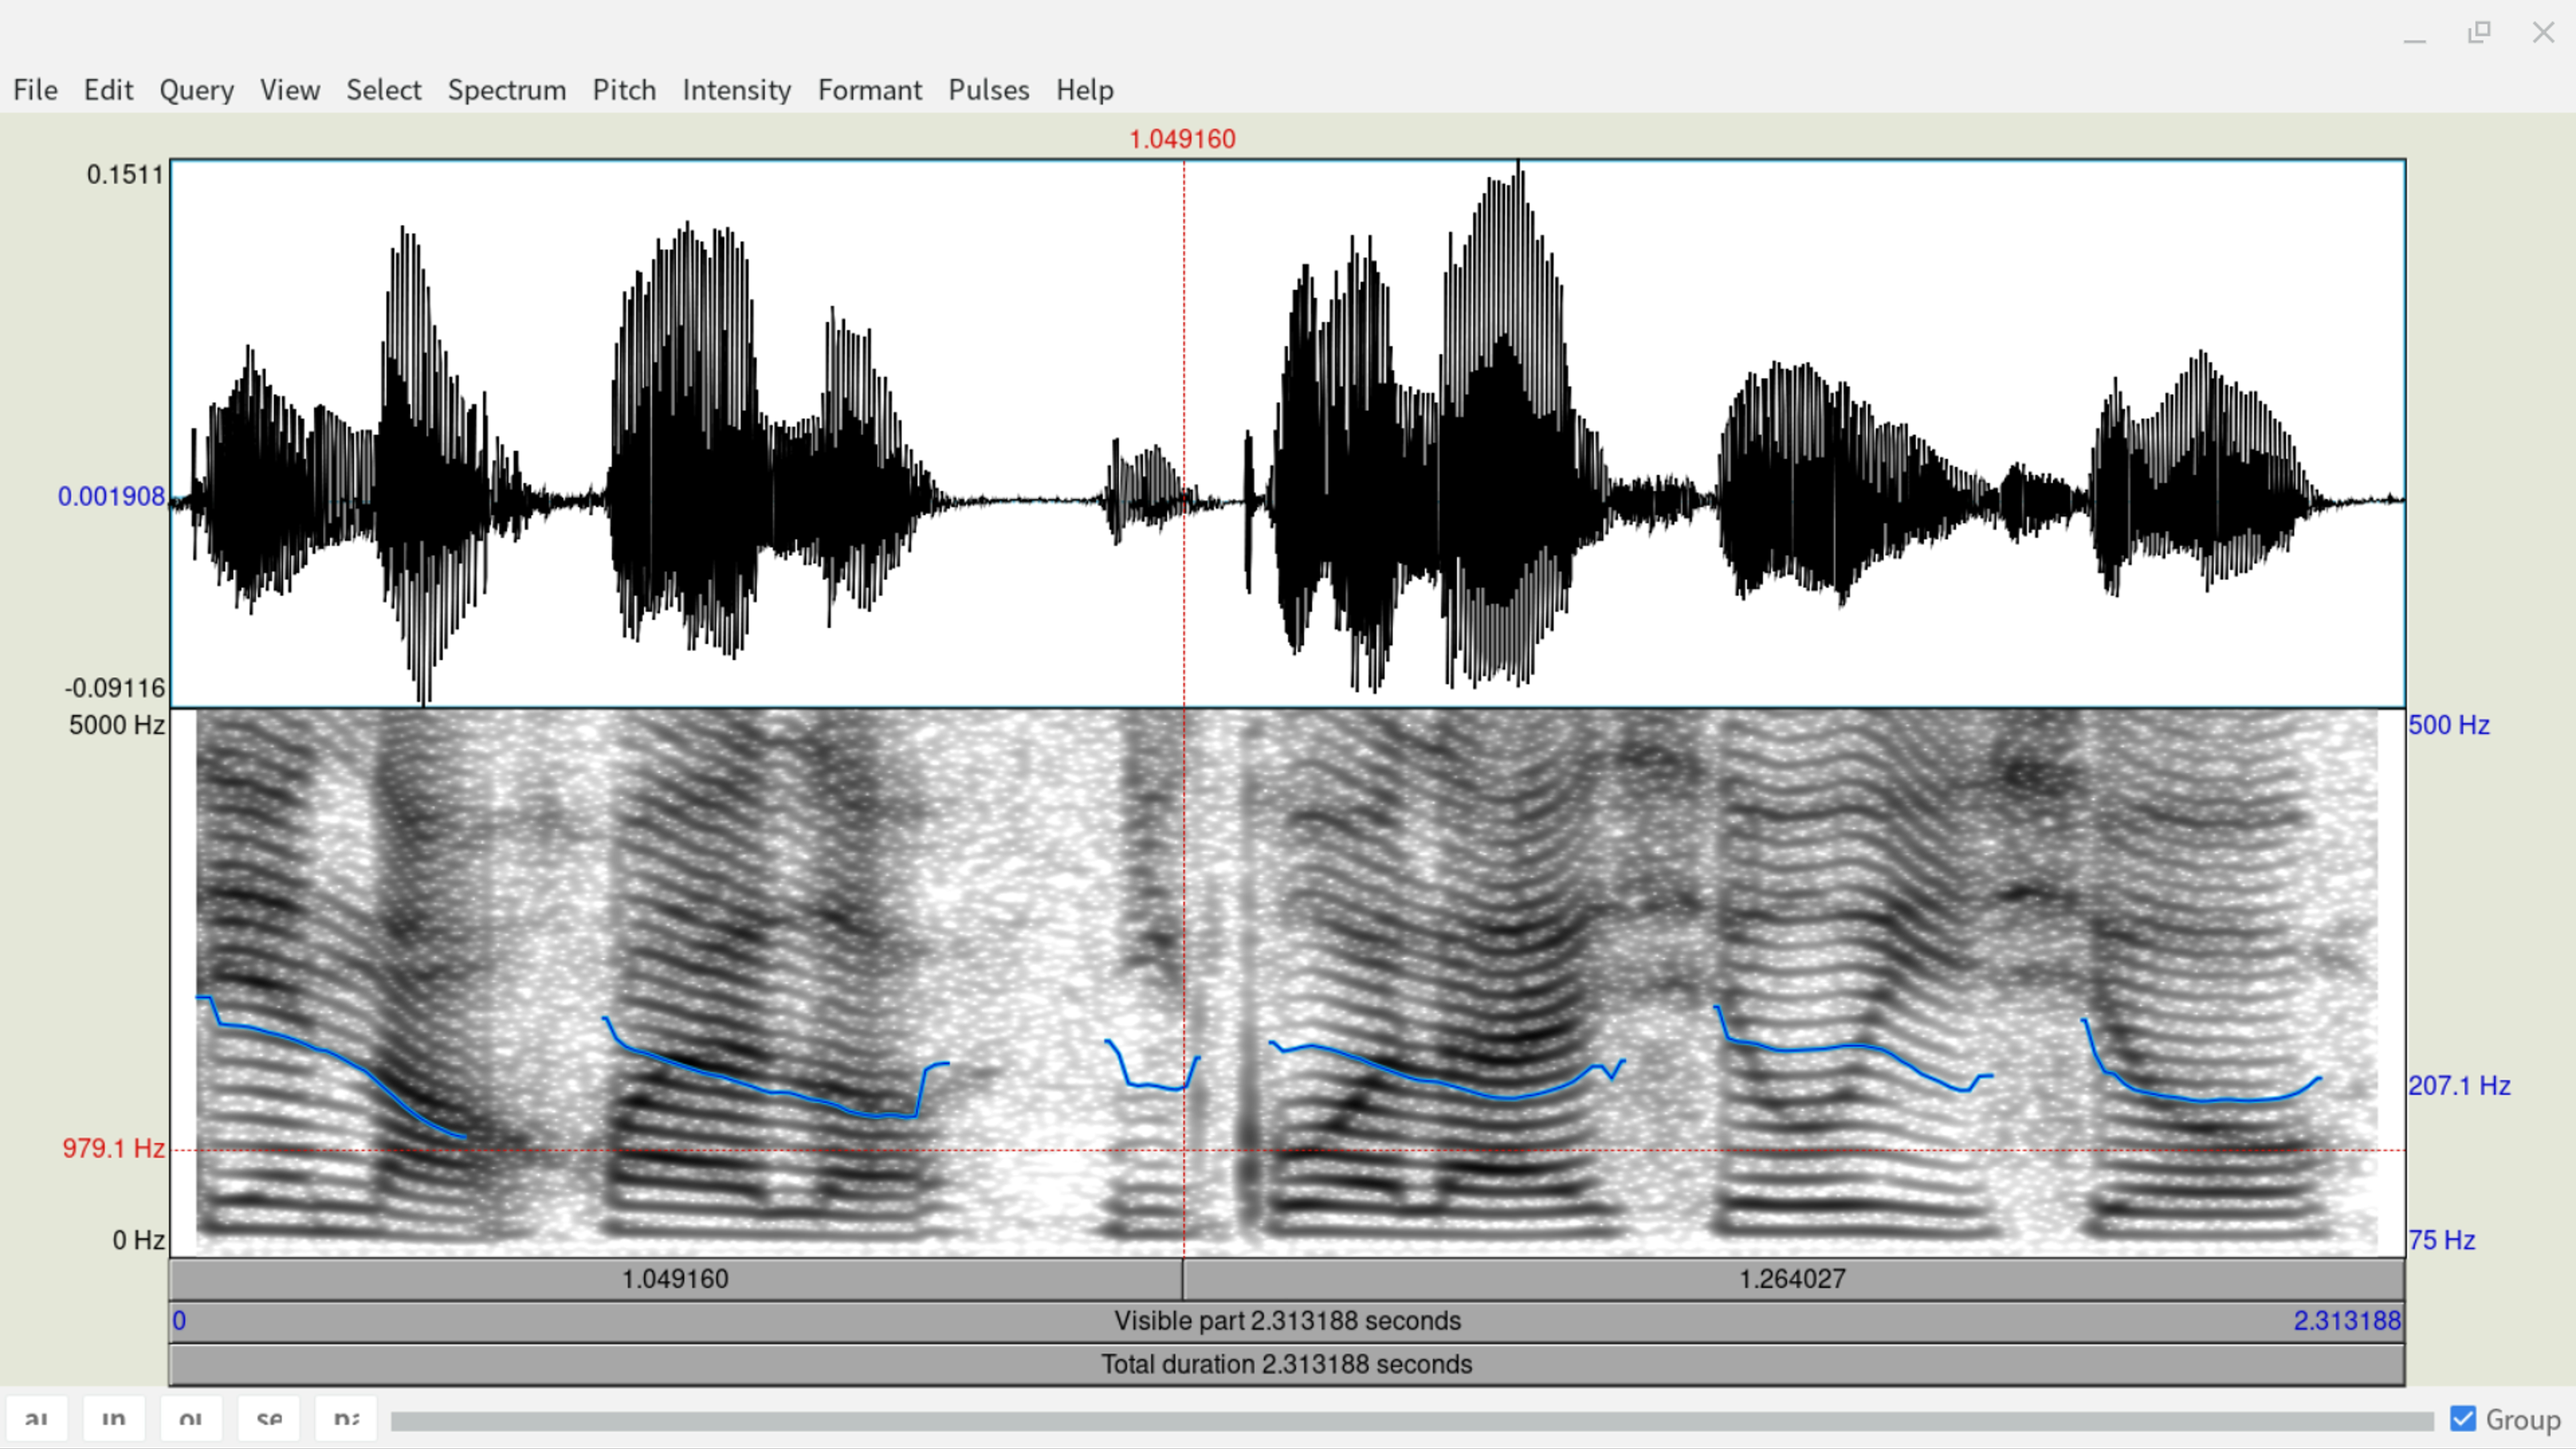
\includegraphics[clip,width=.6\columnwidth]{narrowband.png}%
  }
  \end{center}
  \caption{宽带语谱图和窄带语谱图}
  \label{fig:band}
\end{figure}


\section{宽带语谱图和窄带语谱图}
参考 Praat 官方手册\footnote{\url{https://www.fon.hum.uva.nl/praat/manual/Intro_3_2__Configuring_the_spectrogram.html}}中对宽带语谱图和窄带语谱图的介绍,我们分别设置窗长度为 $5$ ms 和 $30$ ms。
宽带语谱图和窄带语谱图的对比在图~\ref{fig:band}中展示。
两者的差异可概括为:

\begin{enumerate}
  \item \textbf{宽带语谱图}:采用较小的窗口(以及较小的窗移动),这样得出的语谱图的频率分辨率较小,不过时间分辨率较大。频率分辨率较小意味着频带较宽,频率间的区分度较小,具体来说就是语谱图中的条纹之间的分隔不是很明显。不过时间分辨率大,说明不同时间之间的频谱变化可以更加容易被发现。
  \item \textbf{窄带语谱图}:采用较大的窗口(已经较大的窗移动),得到的语谱图的频率分辨率较大,而时间分辨率较小。从图中可以看出窄带语谱图的条纹(频率的能量集中的区域)效果很明显,很容易区分。
\end{enumerate}

\begin{figure}[!htp]
  \centering
  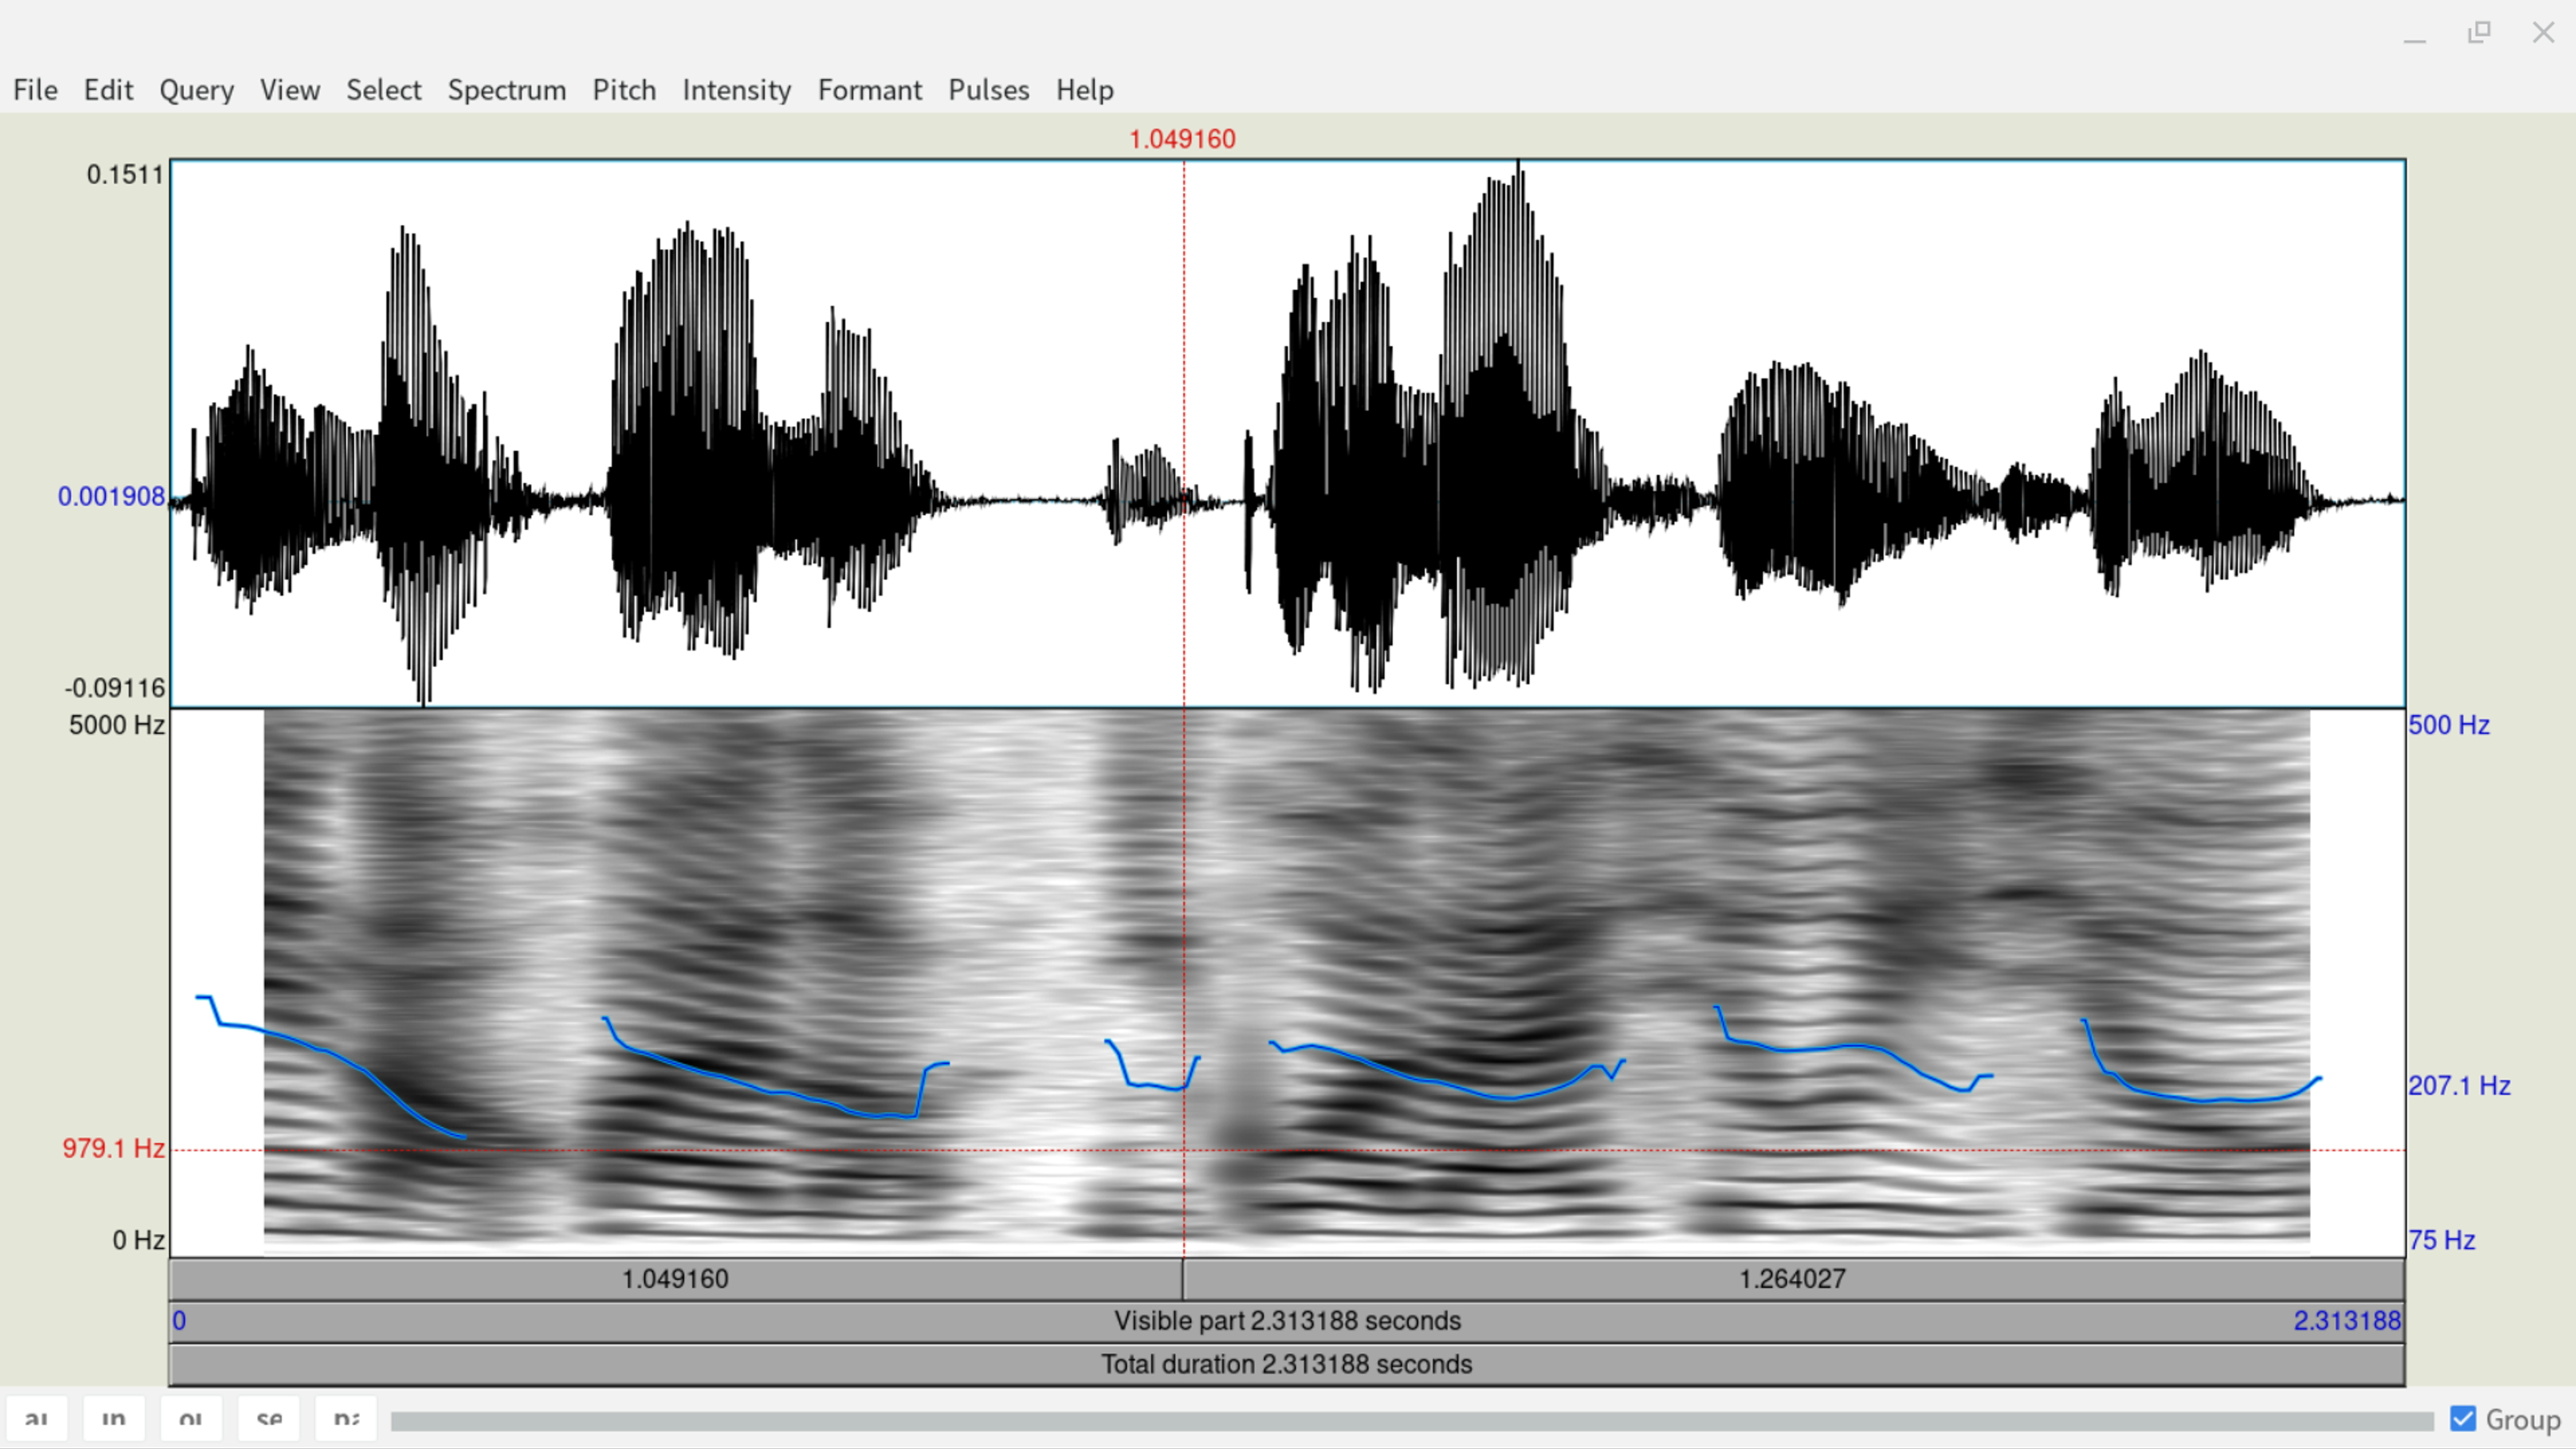
\includegraphics[width=.7\columnwidth]{more_narrowband.png}
  \caption{一个窄带语谱图的例子}
  \label{fig:narrowband}
\end{figure}

可能从 $N = 30$ ms 的窄带语谱图中对于时间分辨率的感知还不够明显,加入我们把窗长调整为 $100$ ms,这时候从图~\ref{fig:narrowband} 中就可以明显感受到,时间方向上,许多频谱变换已经不见了,也就是说过于平滑了以至于丢失了许多细节。

\section{掩蔽效应}

\begin{figure}[!htp]
  \centering
  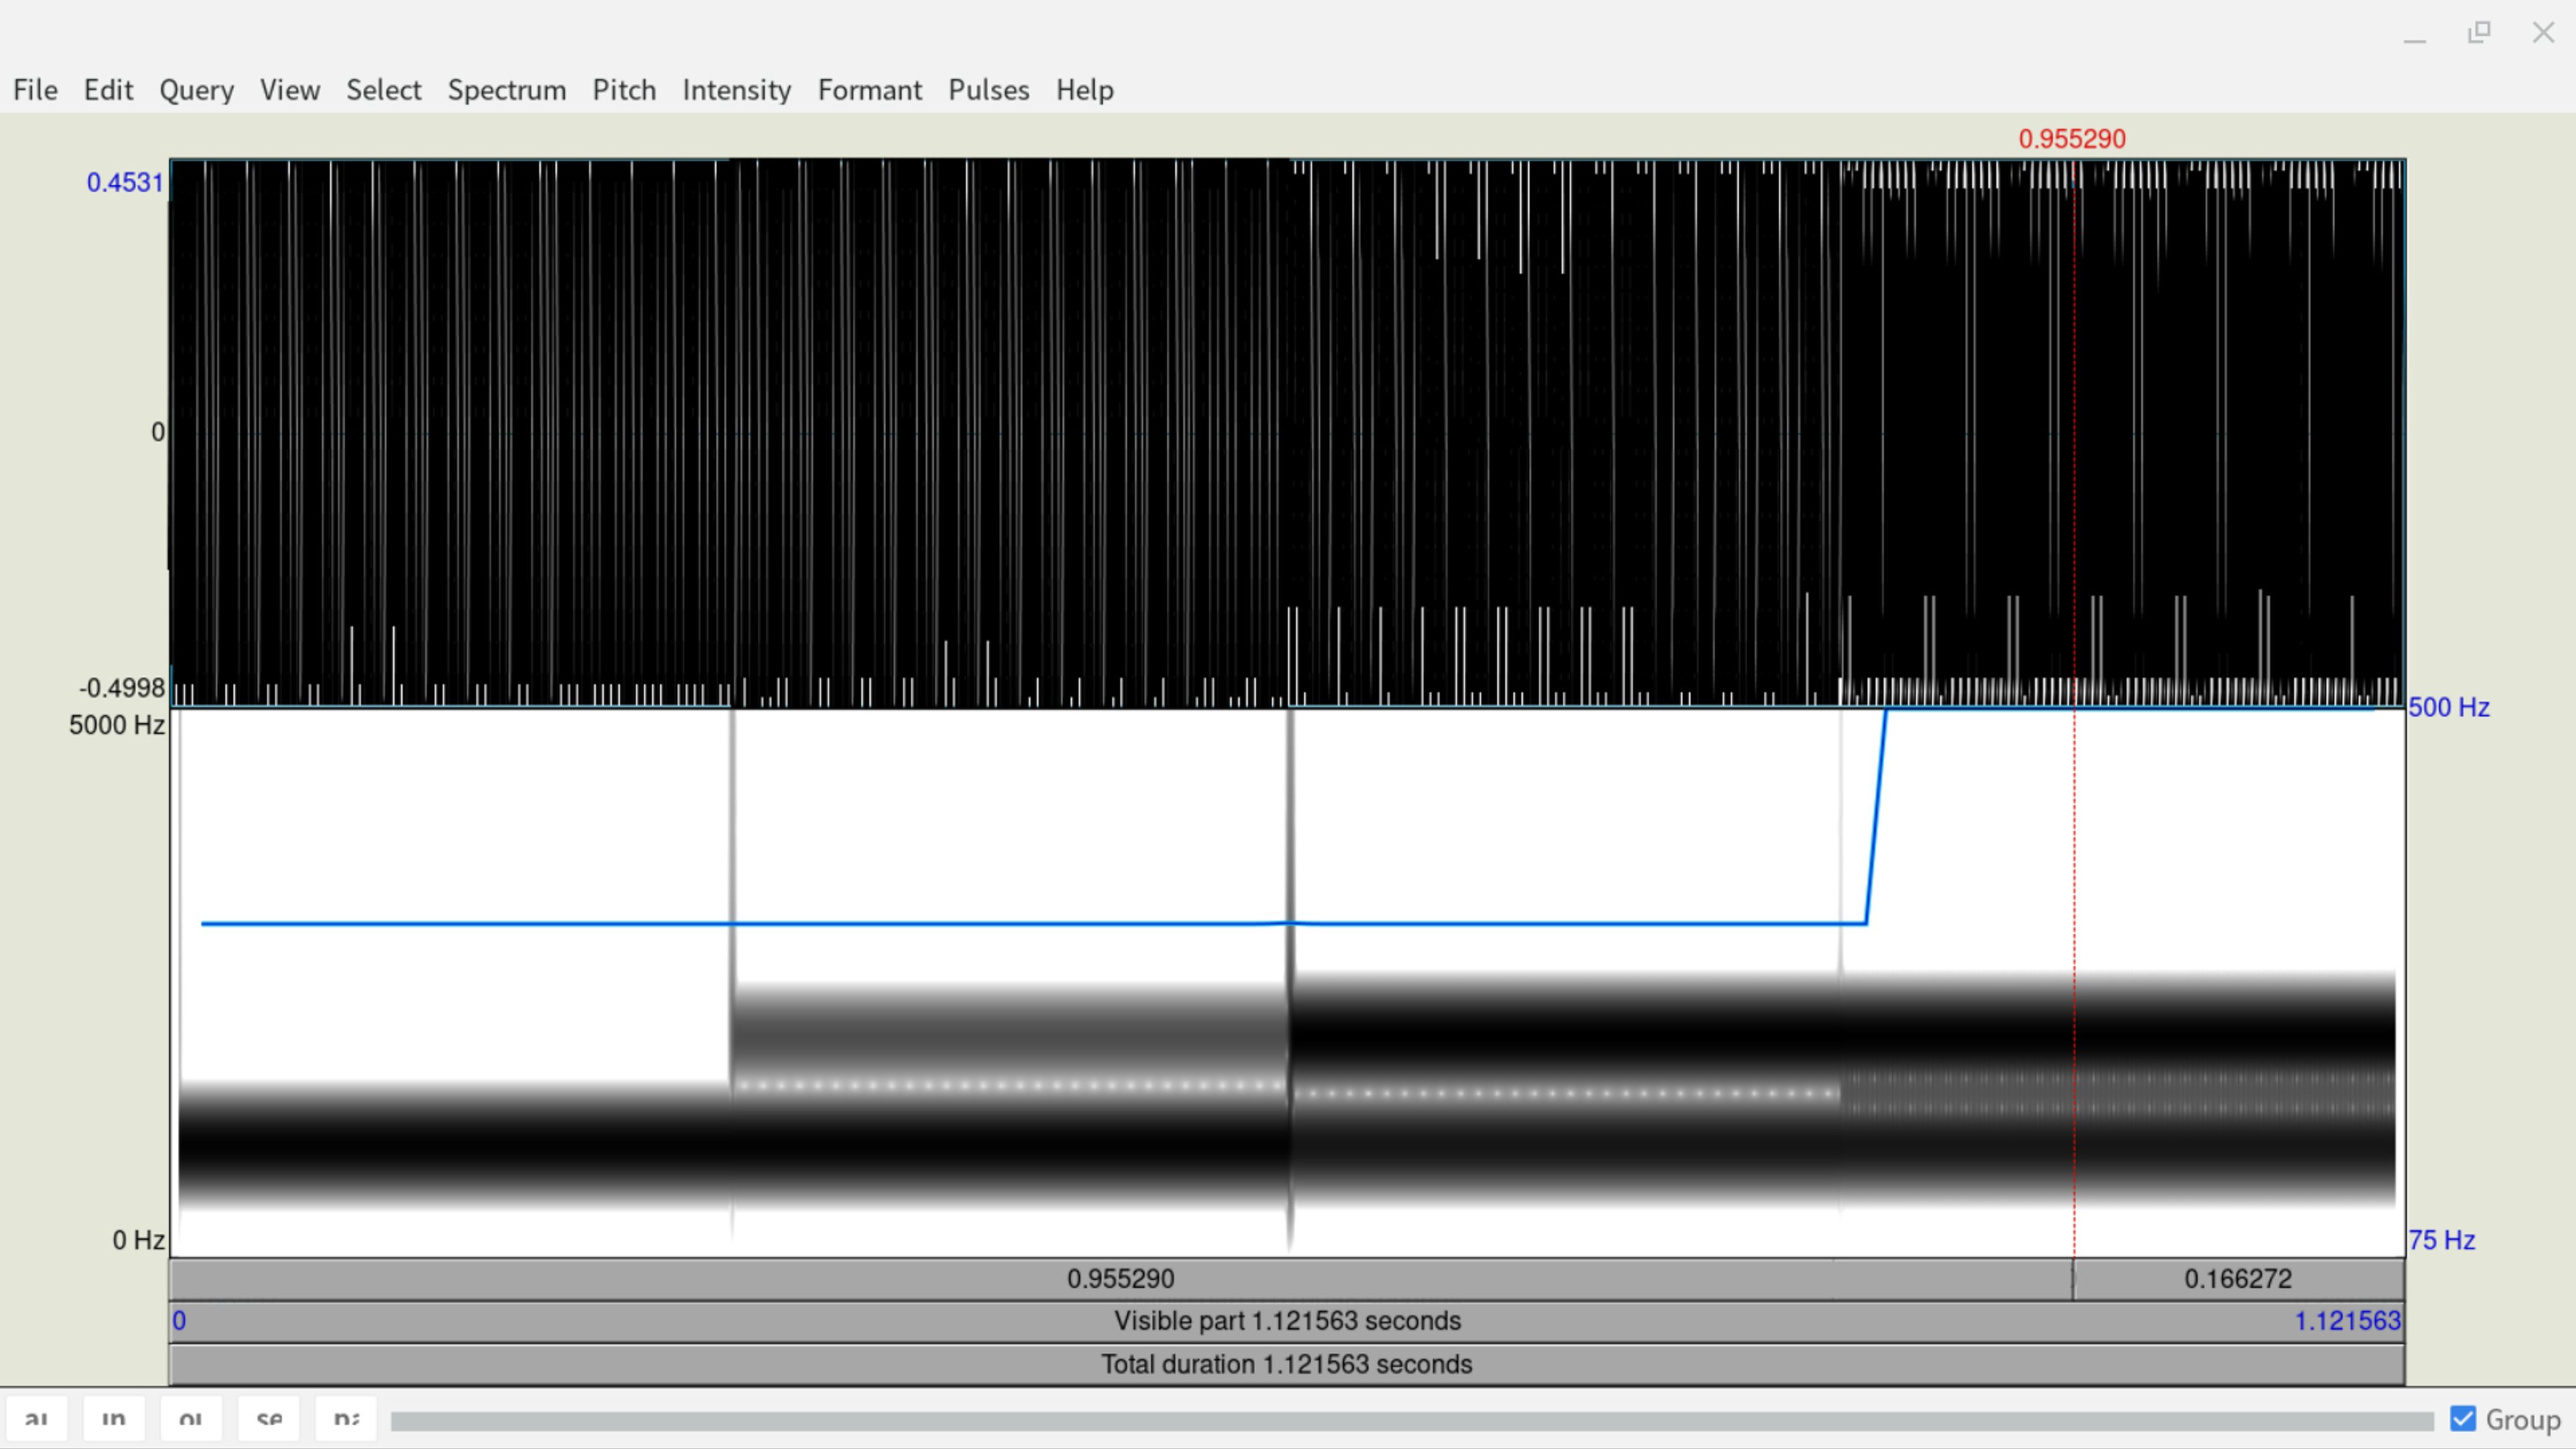
\includegraphics[width=.8\columnwidth]{mask.png}
  \caption{掩蔽效应}
  \label{fig:mask}
\end{figure}

掩蔽效应是一种心理学现象,是由人耳对声音频率分辨机制决定的。是指一个较强声音的附件,相对较弱的声音不易被人耳察觉,即被强音所掩蔽。

图~\ref{fig:mask} 展示了一段用以说明掩蔽效应的声音的波形图和语谱图。
该音频共有四个阶段,第一阶段只有一个频率的声音;第二阶段有两个频率的声音,不过低频能量更大;第三阶段有两个频率,并且他们的能量差不多一样;第四个阶段有三个频率的声音,最低频和最高频的能量相同且较大,而中间频率的能量较小。
对于这四个阶段,我们人耳只能感受出两种声音,也就是第一阶段和第二阶段一样的声音,第三阶段和第四阶段一样的声音。
这是因为低能量的频率被高能量(强音)所掩蔽,这被称为\textbf{同时掩蔽}。
同样的,在时间上相邻的声音之间也有掩蔽现象,被称为\textbf{异时掩蔽}。

